\textcolor{ubuntu_orange}{Centrum Oprogramowania Ubuntu} jest programem służącym do zarządzania zainstalowanymi aplikacjami. W przeciwieństwie do bardziej rozbudowanej klasy programów zwanych Menadżerami pakietów, Centrum Oprogramowania jest swego rodzaju sklepem z aplikacjami. Znajdziesz tutaj gotowe instalatory programów dostępnych w podstawowych repozytoriach a także programy płatne. Z drugiej strony nie ma tutaj pakietów ze składnikami systemu operacyjnego (np. kernel, biblioteki, daemony).

\begin{center}
	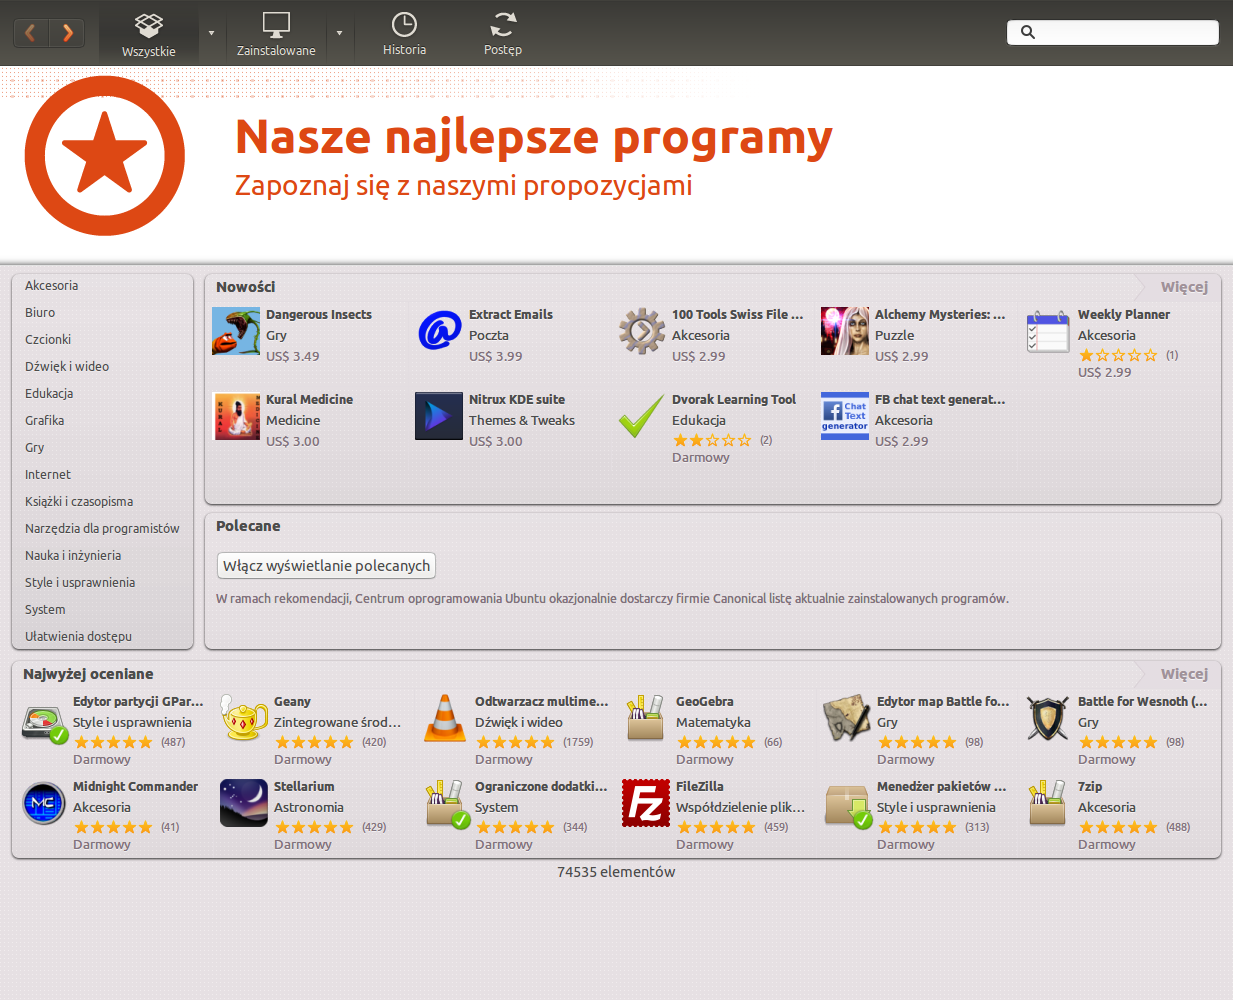
\includegraphics[width=\linewidth]{images/programy_centrum.png}
\end{center} 

W prawym górnym rogu znajduje się pole, w którym możesz wpisać nazwę szukanego programu (lub jej część) a Centrum Oprogramowania ubuntu wyświetli wyniki wyszukiwania. Środkowa część ekranu zawiera polecane i najwyżej oceniane aplikacji. Z lewej strony masz dostęp do kategorii oprogramowania:
\begin{itemize}
\item \textcolor{ubuntu_orange}{Akcesora} zawierają niewielkie programy, pomocne w codziennym użytkowaniu komputera.
\item \textcolor{ubuntu_orange}{Biuro} zawiera programy biurowe, bardziej rozbudowane edytory tekstu, arkusze kalkulacyjne, organizery i inne.
\item \textcolor{ubuntu_orange}{Czcionki} jak sama nazwa wskazuje pozwalają zainstalować dodatkowe zestawy fontów.
\item \textcolor{ubuntu_orange}{Dźwięk i Wideo} zawiera oprogramowanie do tworzenia i odtwarzania multimediów.
\item \textcolor{ubuntu_orange}{Edukacja} to programy wspomagające nauczanie i różnego rodzaju bazy wiedzy.
\item \textcolor{ubuntu_orange}{Grafika} zawiera programy do grafiki wektorowej i rastowej, a także przeglądarki grafiki, programy do wywoływania i korekcji zdjęć.
\item \textcolor{ubuntu_orange}{Gry} zawiera oprogramowanie rozrywkowe.
\item \textcolor{ubuntu_orange}{Internet} zawiera różnego rodzaju oprogramowanie do wymiany danych z internetem (przeglądarki internetowe, klinety poczty email, programy do transmisji danych, klienty Bittorrent).
\item \textcolor{ubuntu_orange}{Książki i Czasopisma} zawierają (najczęściej płatne) publikacje poświęcone Linuksowi i Otwartemu Oprogramowaniu.
\item \textcolor{ubuntu_orange}{Narzędzia dla programistów} to kompilatory, IDE, biblioteki programistyczne i dokumentacja.
\item \textcolor{ubuntu_orange}{Nauka i inżynieria} to programy do komputerowego wspomagania projektowania (CAD).
\item \textcolor{ubuntu_orange}{Style i usprawienia} zawiera zestawy ikon oraz stylów graficznych dla Ubuntu.
\item \textcolor{ubuntu_orange}{System} to narzedzia systemowe, różnego rodzaju konfiguratory.
\item \textcolor{ubuntu_orange}{Ułatwienia dostępu} to programy dla niepełnosprawnych.
\end{itemize}